\setcounter{section}{6}
\section{Quadratische Formen}

Quadratische Gleichungen sind bereits aus der Schulzeit bekannt. In der Regel haben solche Gleichungen in einer Variabel die allgemeine Form:

\begin{equation*}
    f(x) = ax^2 + bx + c.
\end{equation*}

Wie bereits aus der Analysis bekannt, können Gleichungen auch mehr als eine Variable umfassen. Wir werden oft alle Variablen in einem Vektor \( \mathbf{x} = (x_1, \dots, x_n) \) zusammenfassen. Nun können sich auch quadratische Funktionen in mehreren Variablen ergeben. Ein Beispiel hierfür ist eine quadratische Funktion in zwei Variablen:

\begin{equation*}
    q(x_1,x_2) = x_1^2 + 4x_1x_2 + x_2^2.
\end{equation*}

Bei genauerer Betrachtung sieht man, dass diese Funktion auch durch eine Matrix-Vektor Multiplikation beschrieben werden kann. 

\begin{equation*}
    q(x_1, x_2) = \begin{pmatrix} x_1 & x_2 \end{pmatrix} \underbrace{\begin{pmatrix} 1 & 2 \\ 2 & 1 \end{pmatrix}}_{A} \begin{pmatrix} x_1 \\ x_2 \end{pmatrix} = \mathbf{x}^\top A \mathbf{x}.
\end{equation*}

In diesem Fall sagen wir das \( q(\mathbf{x}) = x_1^2 + 4x_1x_2 + x_2^2 \) die quadratische Form der Matrix \( A \) ist. Allgemein können wir für jede symmetrische Matrix \( A \in \mathbb{R}^{n \times n} \), die dazugehörige quadratische Form finden. Sie ist allgemein, wie folgt definiert:

\begin{equation*}
    \begin{aligned}
        q_A: \mathbb{R}^n &\longrightarrow \mathbb{R} \\
        \mathbf{x} &\longmapsto \mathbf{x}^\top A \mathbf{x} = \sum_{i,j=1}^{n} a_{ij}x_i x_j.
    \end{aligned}
\end{equation*}

Für 2 und 3 Dimensionen können wir eine allgemeine Form explizit aufschreiben. 

\begin{equation*}
    \begin{aligned}
        \mathbb{R}^2: q_A(\mathbf{x}) &= \mathbf{x}^\top \begin{pmatrix} a & b \\ b & c \end{pmatrix} \mathbf{x} = ax_1^2 + 2bx_1x_2 + cx_2^2, \\[1em]
        \mathbb{R}^3: q_A(\mathbf{x}) &= \mathbf{x}^\top \begin{pmatrix} a & b & c \\ b & d & e \\ c & e & f \end{pmatrix} \mathbf{x} = ax_1^2 + 2bx_1x_2 + 2cx_1x_3 + dx_2^2 + 2ex_2x_3 + fx_3^2.
    \end{aligned}
\end{equation*}

\vspace{0.25\baselineskip}

Je nach Matrix kann die quadratische Form grafisch anders aussehen. Beispiele für 2 Variablen sind zum Beispiel.

\begin{figure}[h]
    \centering
    \begin{minipage}{0.32\textwidth}
        \centering
        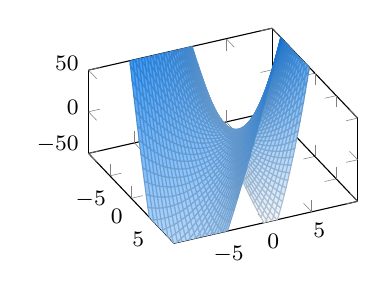
\begin{tikzpicture}
            \begin{axis}[
                tick label style={font=\footnotesize},
                xtick={-5, 0, 5}, 
                ytick={-5, 0, 5},
                width=5cm,
                view={65}{50}, % Adjust the view to come more from the top
                colormap/cool,
                zmin=-50, % Set the minimum value of the z-axis
                zmax=50,  % Set the maximum value of the z-axis
                ]
                \addplot3[
                    surf,
                    domain=-10:10,
                    domain y=-10:10,
                    samples=50,
                ]
                {x^2 + 4*x*y + y^2};
            \end{axis}
        \end{tikzpicture}
    \end{minipage}
    \hfill
    \begin{minipage}{0.32\textwidth}
        \centering
        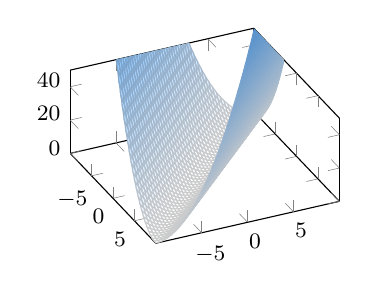
\begin{tikzpicture}
            \begin{axis}[
                width=5cm,
                tick label style={font=\footnotesize},
                xtick={-5, 0, 5}, 
                ytick={-5, 0, 5},
                view={65}{50}, % Adjust the view to come more from the top
                colormap/cool,
                zmin=0, % Set the minimum value of the z-axis
                zmax=50,  % Set the maximum value of the z-axis
                ]
                \addplot3[
                    surf,
                    domain=-10:10,
                    domain y=-10:10,
                    samples=50,
                ]
                {x^2 + 2*x*y + y^2};
            \end{axis}
        \end{tikzpicture}
    \end{minipage}
    \hfill
    \begin{minipage}{0.32\textwidth}
        \centering
        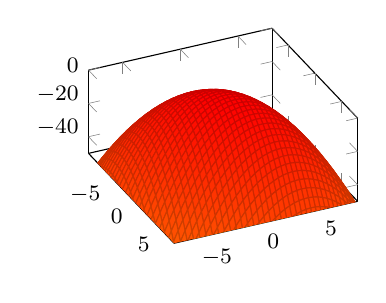
\begin{tikzpicture}
            \begin{axis}[
                tick label style={font=\footnotesize},
                width=5cm,
                view={65}{50}, % Adjust the view to come more from the top
                zmin=-50, % Set the minimum value of the z-axis
                zmax=0,  % Set the maximum value of the z-axis
                ]
                \addplot3[
                    surf,
                    domain=-10:10,
                    domain y=-10:10,
                    samples=50,
                ]
                {-x^2 + x*y - y^2};
            \end{axis}
        \end{tikzpicture}
    \end{minipage}
\end{figure}

\subsection{Definitheit}

Die unterschiedlichen quadratischen Formen und die assoziierten symmetrischen Matrizen lassen sich wie folgt nach Definitheit klassifizieren.

\begin{tcolorbox}[colback=gray!30, colframe=gray!80, title=Definitheit quadratischer Formen]
    Eine quadratische Form, gegeben durch \( q(\mathbf{x}) = \mathbf{x}^\top A \mathbf{x} \), heisst:
    \begin{itemize}
        \item positiv definit: \( \qquad \quad \ q(\mathbf{x}) > 0, \ \forall \mathbf{x} \neq 0 \)
        \item negativ definit: \( \qquad \quad q(\mathbf{x}) < 0, \ \forall \mathbf{x} \neq 0 \)
        \item positiv semidefinit: \( \quad \ q(\mathbf{x}) \geq 0, \ \forall \mathbf{x} \neq 0 \)
        \item negativ semidefinit: \( \quad q(\mathbf{x}) \leq 0, \ \forall \mathbf{x} \neq 0 \)
        \item indefinit: \( \qquad \qquad \qquad \text{sonst} \)
    \end{itemize}

    Die Definitheit kann auch über die Eigenwerte von \( A \) bestimmt werden. Somit ist die Matrix \( A \)
    \begin{itemize}
        \item positiv definit: \( \qquad \quad \ \text{Alle} \ \lambda > 0 \)
        \item negativ definit: \( \qquad \quad \text{Alle} \ \lambda < 0 \)
        \item positiv semidefinit: \( \quad \ \text{Alle} \ \lambda \geq 0 \)
        \item negativ semidefinit: \( \quad \text{Alle} \ \lambda \leq 0 \)
        \item indefinit: \( \qquad \qquad \qquad \text{sonst} \)
    \end{itemize}
\end{tcolorbox}

\vspace{1\baselineskip}

Betrachten wir nochmals die oben gezeigten Beispiele und klassifizieren diese anhand ihrer Definitheit.

\vspace{0.5\baselineskip}

\begin{figure}[h]
    \centering
    \begin{minipage}{0.39\textwidth}
        \centering
        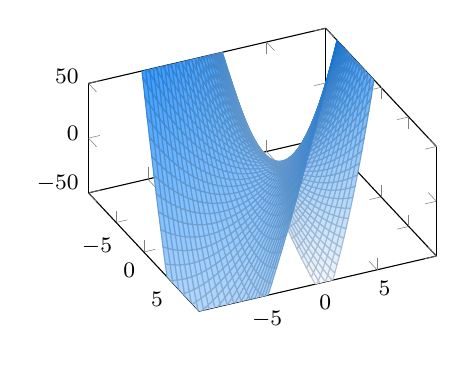
\begin{tikzpicture}
            \begin{axis}[
                tick label style={font=\footnotesize},
                xtick={-5, 0, 5}, 
                ytick={-5, 0, 5},
                width=6cm,
                view={65}{50}, % Adjust the view to come more from the top
                colormap/cool,
                zmin=-50, % Set the minimum value of the z-axis
                zmax=50,  % Set the maximum value of the z-axis
                ]
                \addplot3[
                    surf,
                    domain=-10:10,
                    domain y=-10:10,
                    samples=50,
                ]
                {x^2 + 4*x*y + y^2};
            \end{axis}
        \end{tikzpicture}
    \end{minipage}
    \hfill
    \begin{minipage}{0.6\textwidth}
        \begin{equation*}
            \begin{aligned}
                A = \begin{pmatrix} 1 & 2 \\ 2 & 1 \end{pmatrix} \rightarrow x_1^2 + 4x_1x_2 + x_2^2 \\[0.5em]
                \text{Eigenwerte:} \quad \lambda_1 = 3, \quad \lambda_2 = -1 \\[0.5em]
                \text{Indefinit} \qquad \qquad
            \end{aligned}
        \end{equation*}
    \end{minipage}
\end{figure}

\newpage

\begin{figure}[h]
    \centering
    \begin{minipage}{0.39\textwidth}
        \centering
        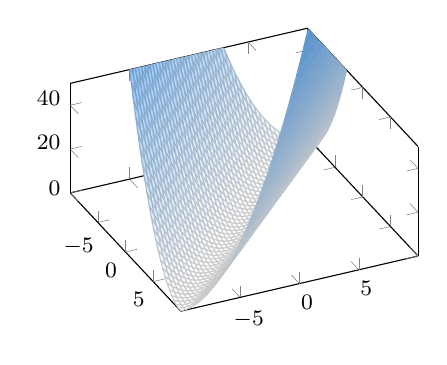
\begin{tikzpicture}
            \begin{axis}[
                tick label style={font=\footnotesize},
                xtick={-5, 0, 5}, 
                ytick={-5, 0, 5},
                width=6cm,
                view={65}{50}, % Adjust the view to come more from the top
                colormap/cool,
                zmin=0, % Set the minimum value of the z-axis
                zmax=50,  % Set the maximum value of the z-axis
                ]
                \addplot3[
                    surf,
                    domain=-10:10,
                    domain y=-10:10,
                    samples=50,
                ]
                {x^2 + 2*x*y + y^2};
            \end{axis}
        \end{tikzpicture}
    \end{minipage}
    \hfill
    \begin{minipage}{0.6\textwidth}
        \begin{equation*}
            \begin{aligned}
                A = \begin{pmatrix} 1 & 1 \\ 1 & 1 \end{pmatrix} \rightarrow x_1^2 + 2x_1x_2 + x_2^2 \\[0.5em]
                \text{Eigenwerte:} \quad \lambda_1 = 2, \quad \lambda_2 = 0 \\[0.5em]
                \text{Positiv semidefinit} \qquad \quad
            \end{aligned}
        \end{equation*}
    \end{minipage}
\end{figure}

\begin{figure}[h]
    \centering
    \begin{minipage}{0.39\textwidth}
        \centering
        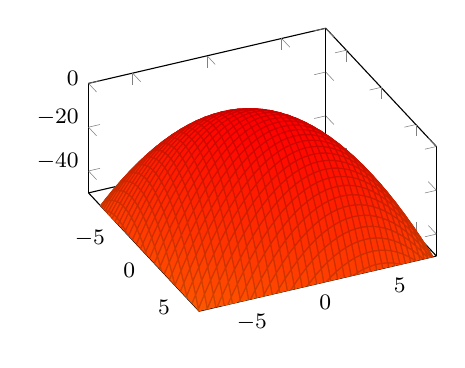
\begin{tikzpicture}
            \begin{axis}[
                tick label style={font=\footnotesize},
                width=6cm,
                view={65}{50}, % Adjust the view to come more from the top
                zmin=-50, % Set the minimum value of the z-axis
                zmax=0,  % Set the maximum value of the z-axis
                ]
                \addplot3[
                    surf,
                    domain=-10:10,
                    domain y=-10:10,
                    samples=50,
                ]
                {-x^2 + x*y - y^2};
            \end{axis}
        \end{tikzpicture}
    \end{minipage}
    \hfill
    \begin{minipage}{0.6\textwidth}
        \begin{equation*}
            \begin{aligned}
                A = \begin{pmatrix} -1 & \frac{1}{2} \\ \frac{1}{2} & -1 \end{pmatrix} \rightarrow -x_1^2 + x_1x_2 - x_2^2 \\[0.5em]
                \text{Eigenwerte:} \quad \lambda_1 = - \frac{3}{2}, \quad \lambda_2 = - \frac{1}{2} \\[0.5em]
                \text{Negativ definit} \qquad \qquad
            \end{aligned}
        \end{equation*}
    \end{minipage}
\end{figure}

\subsection{Rein quadratische Formen}

Eine rein quadratische Form hat keine Mischterme. D.h.\ die Matrix \( A \)  hat nur Diagonaleinträge. Allgemein können wir rein quadratische Formen in dieser Form schreiben

\begin{equation*}
    q_A(\mathbf{x}) = \begin{pmatrix} x_1 & x_2 & \dots & x_n \end{pmatrix} \begin{pmatrix} a_1 & 0 & \dots & 0 \\ 0 & a_2 & \dots & 0 \\ \vdots & \vdots & \ddots & \vdots \\ 0 & 0 & \dots & a_n \end{pmatrix} \begin{pmatrix} x_1 \\ x_2 \\ \vdots \\ x_n \end{pmatrix} = a_1x_1^2 + a_2x_2^2 + \dots + a_nx_n^2.
\end{equation*}

Wie unterscheiden sich rein quadratische Formen von allgemeinen quadratischen Formen? Betrachten wir zwei Beispiele. In einem Fall gibt es Mischterme welche durch Elemente neben der Diagonalen beschrieben werden. Im anderen Fall ist die Matrix diagonal und es gibt keine Mischterme.

\begin{figure}[h]
    \centering
    \begin{minipage}{0.4\textwidth}
        \centering
        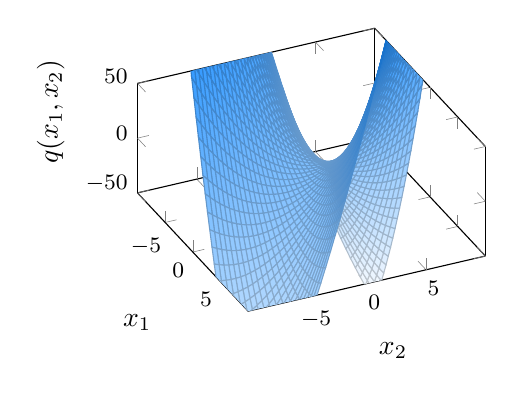
\begin{tikzpicture}
            \begin{axis}[
                tick label style={font=\footnotesize},
                xtick={-5, 0, 5}, 
                ytick={-5, 0, 5},
                width=6cm,
                view={65}{50}, % Adjust the view to come more from the top
                xlabel={$x_1$},
                ylabel={$x_2$},
                zlabel={$q(x_1, x_2)$},
                colormap/cool,
                zmin=-50, % Set the minimum value of the z-axis
                zmax=50,  % Set the maximum value of the z-axis
                ]
                \addplot3[
                    surf,
                    domain=-10:10,
                    domain y=-10:10,
                    samples=50,
                ]
                {x^2 + 4*x*y + y^2};
            \end{axis}
        \end{tikzpicture}
    \end{minipage}
    \hfill
    \begin{minipage}{0.4\textwidth}
        \centering
        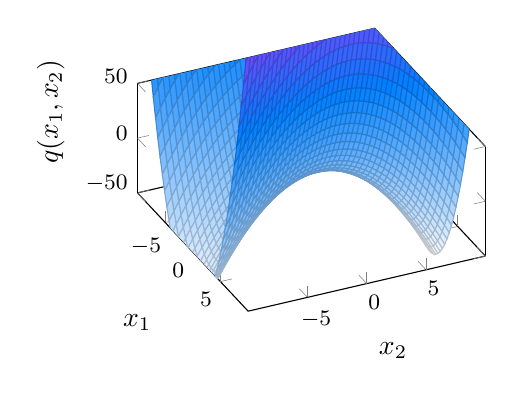
\begin{tikzpicture}
            \begin{axis}[
                tick label style={font=\footnotesize},
                xtick={-5, 0, 5}, 
                ytick={-5, 0, 5},
                width=6cm,
                view={65}{50}, % Adjust the view to come more from the top
                xlabel={$x_1$},
                ylabel={$x_2$},
                zlabel={$q(x_1, x_2)$},
                colormap/cool,
                zmin=-50, % Set the minimum value of the z-axis
                zmax=50,  % Set the maximum value of the z-axis
                xmax=10,
                xmin=-10,
                ]
                \addplot3[
                    surf,
                    domain=-10:10,
                    domain y=-10:10,
                    samples=50,
                ]
                {3*x^2 - y^2};
            \end{axis}
        \end{tikzpicture}
    \end{minipage}
\end{figure}

\newpage

\begin{figure}[h]
    \centering
    \begin{minipage}{0.4\textwidth}
        \centering
        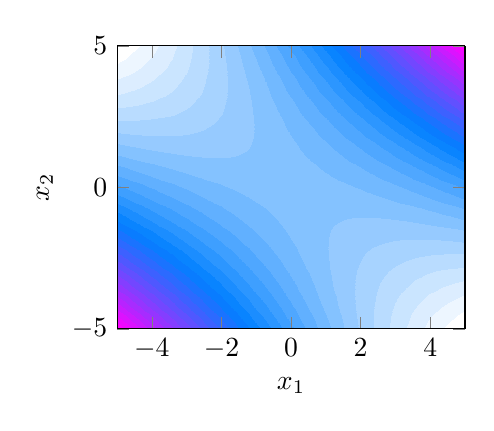
\begin{tikzpicture}
            \begin{axis}[
                width=6cm,
                xlabel={$x_1$},
                ylabel={$x_2$},
                colormap/cool,
                view={0}{90},
                ]
                \addplot3[
                    contour filled={
                        number=30, % Number of contour levels
                    },
                    domain=-5:5,
                    domain y=-5:5,
                    samples=75,
                ]
                {x^2 + 4*x*y + y^2};
            \end{axis}
        \end{tikzpicture}
    \end{minipage}
    \hfill
    \begin{minipage}{0.4\textwidth}
        \centering
        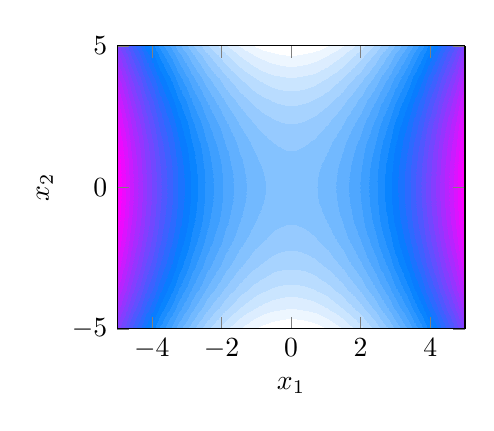
\begin{tikzpicture}
            \begin{axis}[
                width=6cm,
                xlabel={$x_1$},
                ylabel={$x_2$},
                colormap/cool,
                view={0}{90},
                ]
                \addplot3[
                    contour filled={
                        number=30, % Number of contour levels
                    },
                    domain=-5:5,
                    domain y=-5:5,
                    samples=75,
                ]
                {3*x^2 - y^2};
            \end{axis}
        \end{tikzpicture}
    \end{minipage}
\end{figure}

\begin{equation*}
    \begin{aligned}
        A = \begin{pmatrix} 1 & 2 \\ 2 & 1 \end{pmatrix} \qquad \qquad \qquad \qquad \qquad \qquad \qquad A = \begin{pmatrix} 3 & 0 \\ 0 & -1 \end{pmatrix}
    \end{aligned}
\end{equation*}

\vspace{0.5\baselineskip}

Es scheint hier als ob die beiden Formen dieselbe Fläche beschreiben mit dem einzigen Unterschied, dass sie rotiert sind. In folgenden Kapiteln werden wir sehen wie wir durch eine Basistransformation eine nicht reine Form in eine rein quadratische Form umwandeln können. Dafür werden wir das Konzept der Diagonalisierung verwenden. 